%%%%%%%%%%%%%%%%%%%%%%%%%%%%%%%%%%%%%%%%%%%%%%%%%%%%%%%%%%%%%%%%%
% MUW Presentation
% LaTeX Template
% Version 1.0 (27/12/2016)
%
% License:
% CC BY-NC-SA 4.0 (http://creativecommons.org/licenses/by-nc-sa/3.0/)
%
% Created by:
% Nicolas Ballarini, CeMSIIS, Medical University of Vienna
% nicoballarini@gmail.com
% http://statistics.msi.meduniwien.ac.at/
%
% Customized for UAH by:
% David F. Barrero, Departamento de Automática, UAH
%%%%%%%%%%%%%%%%%%%%%%%%%%%%%%%%%%%%%%%%%%%%%%%%%%%%%%%%%%%%%%%%%

\documentclass[10pt,compress]{beamer} % Change 10pt to make fonts of a different size
\mode<presentation>

\usepackage[spanish]{babel}
\usepackage{fontspec}
\usepackage{tikz}
\usepackage{etoolbox}
\usepackage{xcolor}
\usepackage{xstring}
\usepackage{listings}

% Custom packages
\usepackage{tikz}
\def\layersep{2.5cm}
\usetikzlibrary{matrix,chains,positioning,decorations.pathreplacing,arrows}

\usetheme{UAH}
\usecolortheme{UAH}
\setbeamertemplate{navigation symbols}{} 
\setbeamertemplate{caption}[numbered]

%%%%%%%%%%%%%%%%%%%%%%%%%%%%%%%%%%%%%%%%%%%%%%%%%%%%%%%%%%%%%%%%%
%% Presentation Info
\title[AI in videogames]{AI in videogames}
\author{\asignatura\\\carrera}
\institute{}
\date{Departamento de Automática}
%%%%%%%%%%%%%%%%%%%%%%%%%%%%%%%%%%%%%%%%%%%%%%%%%%%%%%%%%%%%%%%%%


%%%%%%%%%%%%%%%%%%%%%%%%%%%%%%%%%%%%%%%%%%%%%%%%%%%%%%%%%%%%%%%%%
%% Descomentar para habilitar barra de navegación superior
\setNavigation
%%%%%%%%%%%%%%%%%%%%%%%%%%%%%%%%%%%%%%%%%%%%%%%%%%%%%%%%%%%%%%%%%

%%%%%%%%%%%%%%%%%%%%%%%%%%%%%%%%%%%%%%%%%%%%%%%%%%%%%%%%%%%%%%%%%
%% Configuración de logotipos en portada
%% Opacidad de los logotipos
\newcommand{\opacidad}{1}
%% Descomentar para habilitar logotipo en pié de página de portada
\renewcommand{\logoUno}{Images/isg.png}
%% Descomentar para habilitar logotipo en pié de página de portada
%\renewcommand{\logoDos}{Images/CCLogo.png}
%% Descomentar para habilitar logotipo en pié de página de portada
%\renewcommand{\logoTres}{Images/ALogo.png}
%% Descomentar para habilitar logotipo en pié de página de portada
%\renewcommand{\logoCuatro}{Images/ELogo.png}
%%%%%%%%%%%%%%%%%%%%%%%%%%%%%%%%%%%%%%%%%%%%%%%%%%%%%%%%%%%%%%%%%

%%%%%%%%%%%%%%%%%%%%%%%%%%%%%%%%%%%%%%%%%%%%%%%%%%%%%%%%%%%%%%%%%
%% FOOTLINE
%% Comment/Uncomment the following blocks to modify the footline
%% content in the body slides. 


%% Option A: Title and institute
\footlineA
%% Option B: Author and institute
%\footlineB
%% Option C: Title, Author and institute
%\footlineC
%%%%%%%%%%%%%%%%%%%%%%%%%%%%%%%%%%%%%%%%%%%%%%%%%%%%%%%%%%%%%%%%%

\begin{document}

%%%%%%%%%%%%%%%%%%%%%%%%%%%%%%%%%%%%%%%%%%%%%%%%%%%%%%%%%%%%%%%%%
% Use this block for a blue title slide with modified footline
{\titlepageBlue
    \begin{frame}
        \titlepage
    \end{frame}
}

\institute{\asignatura}

\begin{frame}[plain]{}
   \begin{block}{Objectives}
       \begin{itemize}
        \item Introduce the role of AI in videogames
        \item Describe the main AI methods used in videogames
       \end{itemize}
   \end{block}

   \begin{block}{Bibliography}
       \textit{Desarrollo de Videojuegos. Desarrollo de componentes}. Capítulo 1. UCLM.
   \end{block}
\end{frame}

{
\disableNavigation{white}
\begin{frame}[shrink]{Table of Contents}
 \frametitle{Table of Contents}
 \tableofcontents
  % You might wish to add the option [pausesections]
\end{frame}
}

\section{Introduction}

\begin{frame}{Introduction}
    \begin{columns}
	\vspace{-0.5cm}
 	   \column{.90\textwidth}
		\vspace{-0.5cm}
		\begin{block}{What is AI?}
		AI is about making computers able to perform the thinking tasks that humans and animals are capable of.\\
		\raggedleft{ \textit{I. Millington, ``AI for games''}}
		\end{block}
	\end{columns}
		\vspace{0.25cm}
	AI is a key component in any videogame: \alert{Emotional stimulus}
	\begin{itemize}
		\item AI provides a challenge
		\item Hard enough to be a challenge ...
		\item ... easy enough to avoid frustration
  	\end{itemize}
	AI in videogames aims to give fun
	\begin{itemize}
		\item Classical AI seeks optimal solutions
		\item AI in videogames optimizes fun: Realistic behavior
  	\end{itemize}
\end{frame}

\section{Basic concepts}
\subsection{Turing test}
\begin{frame}{Basic concepts}{Turing test}
	   Turing test: Is a person able to distinguish between another person and an AI?\\
		\centering{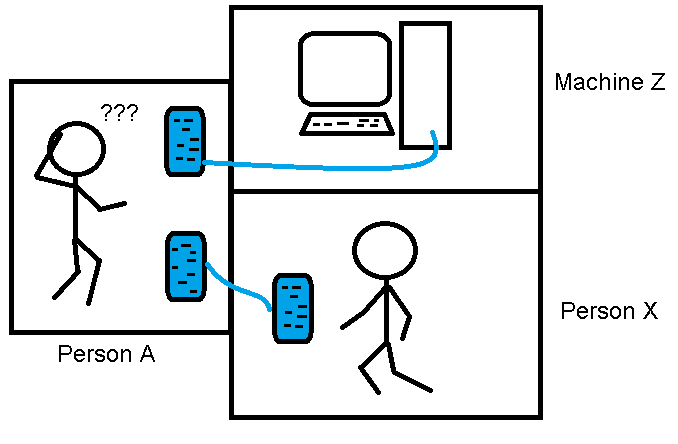
\includegraphics[width=0.35\linewidth]{figs/turing-test}\hspace{0.5cm}
		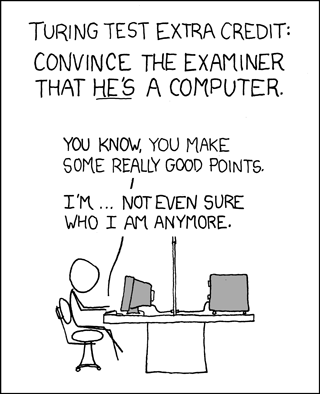
\includegraphics[width=0.2\linewidth]{figs/turingtestjoke}}\\
		\raggedright Turing test in videogames: Does an AI play like a human?
 	 	\begin{itemize}
		\item Chess games, shooters, etc
		\end{itemize}
		Better AI with more computational resources
 	 	\begin{itemize}
		\item Computational resources are limited
		\end{itemize}
\end{frame}

\subsection{Intelligence illusion}
\begin{frame}{Basic concepts}{Intelligence illusion}
	Balance between intelligence and computational resources
  	\begin{itemize}
		\item Intelligence, in videogames, is subjective
		\item AI in videogames seeks \alert{intelligence illusion}
	\end{itemize}
	Many na\"ive (yet very useful) techniques
	\begin{itemize}
		\item Modify NPC state: More life, stamina or speed
		\item Damage vs. impact point
	\end{itemize}
	\begin{center}
		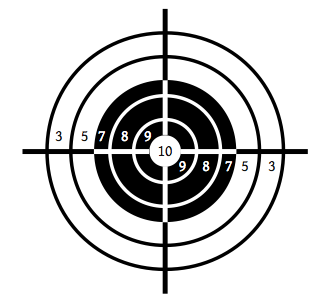
\includegraphics[width=0.2\linewidth]{figs/diana}
		\vspace{1cm}
		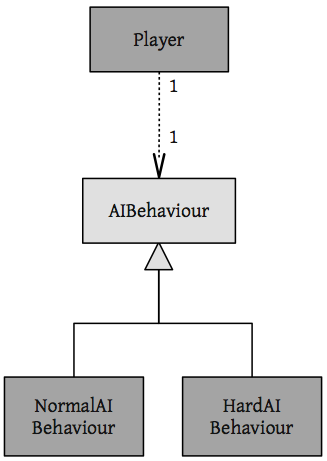
\includegraphics[width=0.15\linewidth]{figs/halo}
	\end{center}
\end{frame}

\subsection{Complexity fallacy}
\begin{frame}{Basic concepts}{Complexity fallacy}
	Complex behaviors are better?
  	\begin{itemize}
		\item Good AI matches the right behavior to the right algorithm
	\end{itemize}
	Study case: Pac-Mac
	\begin{itemize}
		\item Ghosts with two states: normal and frightened (FSM)
		\item In normal state ghosts moves in a straight line
		\item When finds a junction semi-randomly chooses a route
		\begin{itemize}
			\item Blinky (red): Follows Pac-Man (no path-planning)
			\item Pinky (pink): Goes to four tiles ahead Pac-Man
			\item Inky (blue): Takes Pac-Man and Blinky's positions
			\item Clyde (orange): Random
		\end{itemize}
	\end{itemize}
	\begin{center}
		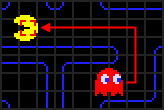
\includegraphics[width=0.15\linewidth]{figs/red}\hspace{0.5cm}
		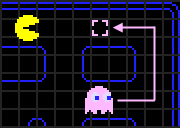
\includegraphics[width=0.15\linewidth]{figs/pink}\hspace{0.5cm}
		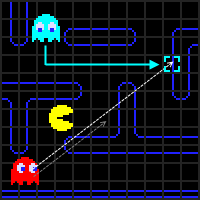
\includegraphics[width=0.15\linewidth]{figs/blue}\hspace{0.5cm}
		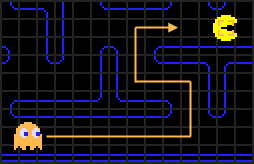
\includegraphics[width=0.15\linewidth]{figs/orange}
	\end{center}
\end{frame}

\section{AI in videogames}
\subsection{Main AI applications}
\begin{frame}{AI in videogames}{Main AI applications}
    \begin{columns}
	\vspace{-0.5cm}
 	   \column{.50\textwidth}
	   Main applications
	   \begin{itemize}
			\item NPC control
			\item Path-planning \href{http://qiao.github.io/PathFinding.js/visual/}{(Demo)}
			\item Search and planning
		\end{itemize}

 	   \column{.50\textwidth}
	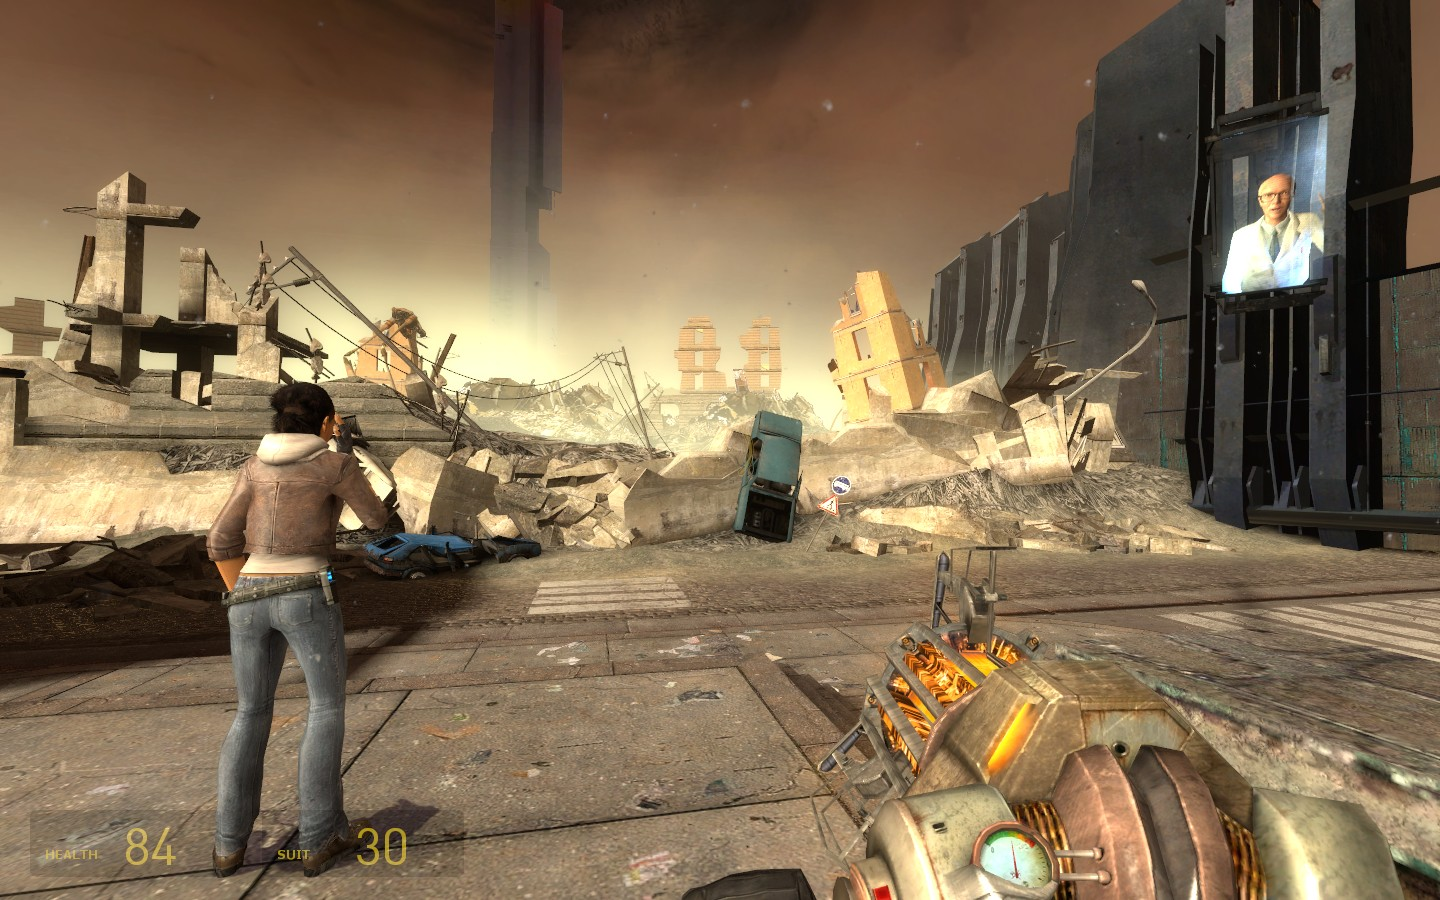
\includegraphics[width=0.8\linewidth]{figs/hl2}\\
	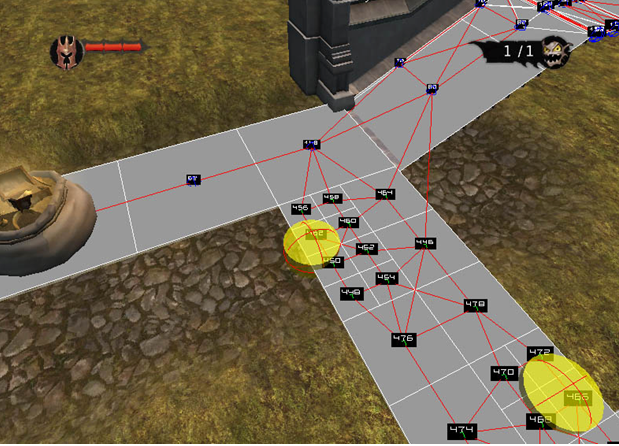
\includegraphics[width=0.8\linewidth]{figs/pp}\\
	\end{columns}
\end{frame}

\subsection{Advanced AI applications}
\begin{frame}{AI in videogames}{Advanced AI applications}
    \begin{columns}
	\vspace{-0.5cm}
 	   \column{.50\textwidth}
	   Advanced applications:
	   \begin{itemize}
			\item NPC behavior learning
			\item Player modeling
			\item Games as AI benchmarks
			\item Procedural-content generation
			\item Computational narrative
			\item Believable agents
			\item AI-assisted game design
		\end{itemize}
 	   \column{.50\textwidth}

	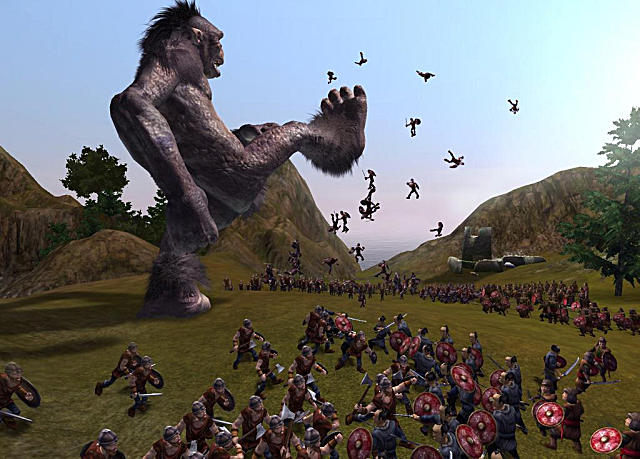
\includegraphics[width=0.8\linewidth]{figs/bw}\\
	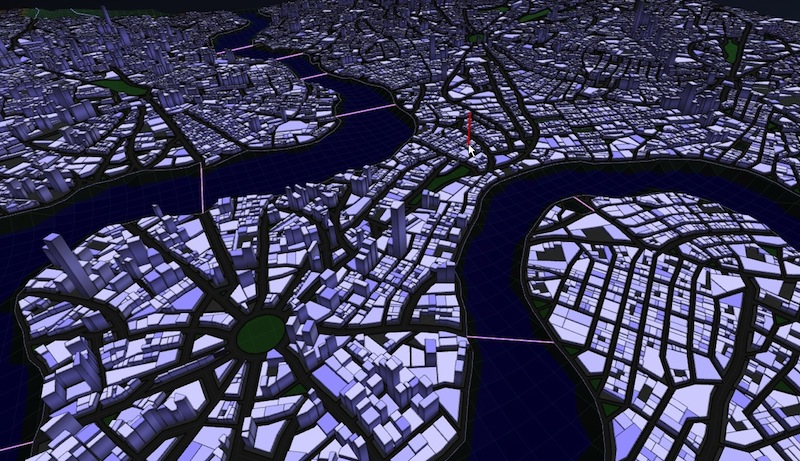
\includegraphics[width=0.8\linewidth]{figs/procedural}
	\end{columns}
\end{frame}


\section{Model of AI}
\subsection{Overview}
\begin{frame}{Model of AI}{Overview}
    \begin{columns}
	  	   \column{.30\textwidth}
		\begin{itemize}
		\item Movement
		\item Decision making
		\item Strategy
		\item Infrastructure
		\end{itemize}
 	   \column{.70\textwidth}
		\centering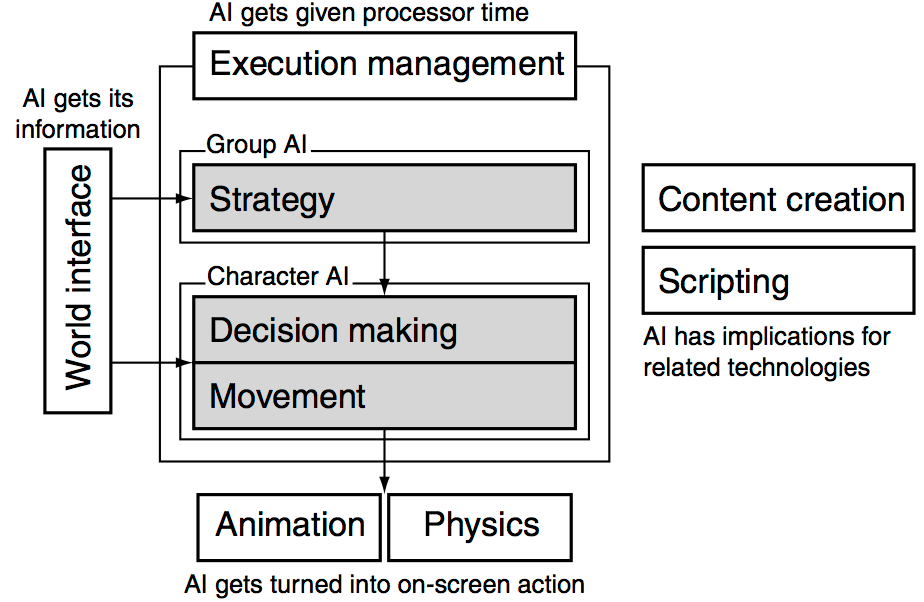
\includegraphics[width=\linewidth]{figs/aimodel}\\

	\end{columns}
\end{frame}

\subsection{Details}
\begin{frame}{Model of AI}{Details}
	\begin{itemize}
	\item \textbf{Movement}: Algorithms that turn decisions into motion
	\begin{itemize}
		\item How to move from point A to point B?: Path-planning algorithms
	\end{itemize}
	\item \textbf{Decision making}: What to do next?
	\begin{itemize}
		\item Each NPC has a range of actions: Attacking, hiding, exploring, patroling, ...
		\item Select the action
		\item Implementation done with movement and animations
	\end{itemize}
	\item \textbf{Strategy}: Team coordination
	\begin{itemize}
		\item Group decision making ...
		\item ... even though each individual makes its own decision
	\end{itemize}
	\item \textbf{Infrastructure}: Support features
	\begin{itemize}
		\item Perception, interfaces to animation and physics engine, etc
		\item Resources management
	\end{itemize}
	\end{itemize}
\end{frame}

\section{Basic AI techniques in videogames}
\subsection{Overview}
\begin{frame}{Basic AI techniques in videogames}{Overview}
	Basic techniques
 	\begin{itemize}
 		\item Classic search algorithms
		\item Finite State Machines
 	\end{itemize}
	
	Advanced techniques
 	\begin{itemize}
 		\item Agents
		\item Fuzzy logic
		\item Artificial Neural Networks
		\item Genetic Algorithms
 	\end{itemize}
	
\end{frame}

\subsection{Search algorithms}
\begin{frame}{AI techniques in videogames}{Search algorithms (I)}
	Almost any problem in AI is a search problem
		\begin{itemize}
		\item Search the best path
		\item Search the best attack
		\item Search the best strategy
		\item Search the best move
		\end{itemize}
	Any AI search algorithm can be used
		\begin{itemize}
		\item A*, Minimax, Depth-first, Dijkstra, ... 
		\end{itemize}
	The issue is to express the problem in terms of a search task
\end{frame}

\begin{frame}{Basic AI techniques in videogames}{Search algorithms (II)}
    \begin{columns}
 	   \column{.60\textwidth}
		\centering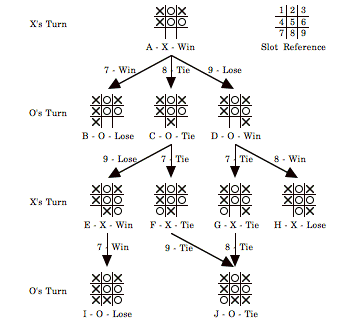
\includegraphics[width=\linewidth]{figs/tree}
 	   \column{.40\textwidth}
		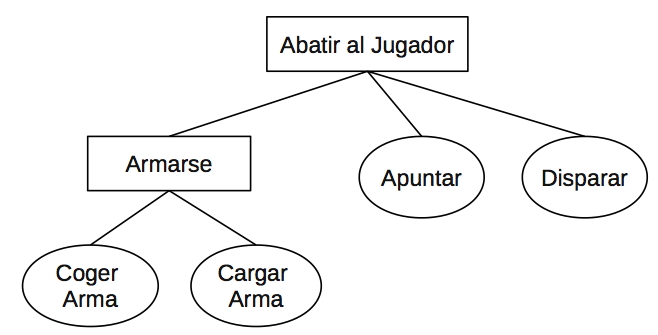
\includegraphics[width=\linewidth]{figs/tree2}
	\end{columns}
\end{frame}

\subsection{Finite State Machines (FSM)}
\begin{frame}{Basic AI techniques in videogames}{Finite State Machines (FSM) (I)}
    \begin{columns}
 	   \column{.50\textwidth}
	   \begin{block}{}
	   	A FSM contains a set of states, transitions and triggering events that rules the transitions
		\end{block}
 	   \column{.50\textwidth}
		Features:
		\begin{itemize}
		\item Easy and fast method
		\item Easy debugging
		\item Intuitive
		\item Flexible
		\end{itemize}
	\end{columns}
	\vspace{0.5cm}
		\centering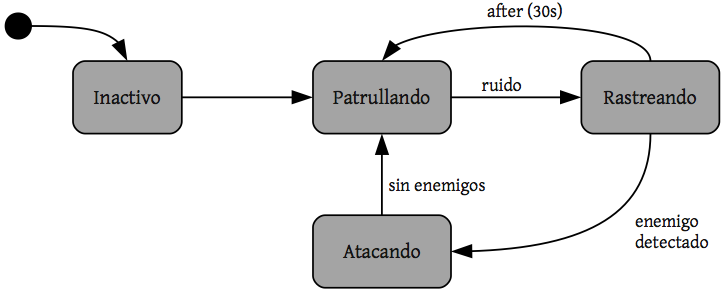
\includegraphics[width=0.7\linewidth]{figs/fsm}\\
\end{frame}

\begin{frame}{Basic AI techniques in videogames}{Finite State Machines (FSM) (II)}
		\centering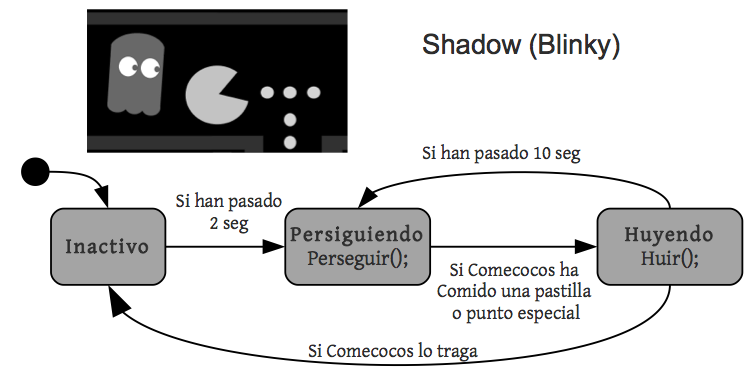
\includegraphics[width=0.8\linewidth]{figs/fsmpacman}\\
\end{frame}

\section{Advanced AI techniques in videogames}
\subsection{Agents}
\begin{frame}{Advanced AI techniques in videogames}{Agents}
    \begin{columns}
 	   \column{.50\textwidth}
	   \vspace{-0.8cm}
		\begin{block}{Agent definition}
		An agent is an goal-oriented entity able to perceive its environment and act on it
		\end{block}
 	   \column{.50\textwidth}
		Agent properties
		\begin{itemize}
		\item Autonomy
		\item Social skills
		\item Reactivity
		\item Proactivity
		\end{itemize}
	\end{columns}
		Related concepts: Learning and reasoning\\
		\vspace{0.5cm}
		\centering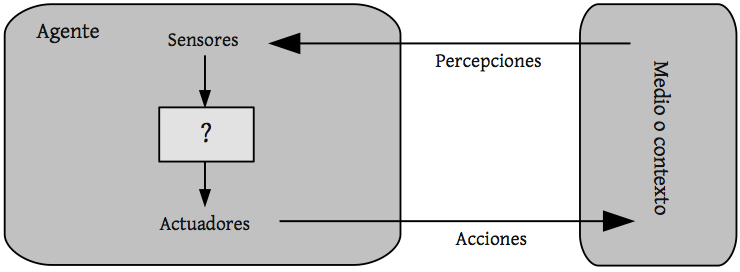
\includegraphics[width=0.7\linewidth]{figs/agent}\\
\end{frame}

\subsection{Fuzzy logic}
\begin{frame}{Advanced AI techniques in videogames}{Fuzzy logic (I)}
    \begin{columns}
 	   \column{.50\textwidth}
	   \vspace{-0.8cm}
		\begin{block}{Fuzzy logic}
		Fuzzy logic, in opposition to digital logic, considers different levels of truee values
		\end{block}
 	   \column{.50\textwidth}
		Properties
		\begin{itemize}
		\item Closer to human reasoning
		\item A fact can be true and false
		\item Deals with imprecise linguistic terms
		\end{itemize}
	\end{columns}

		\centering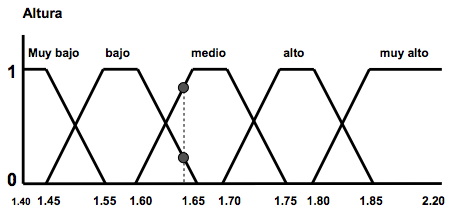
\includegraphics[width=0.6\linewidth]{figs/fuzzy}\\
\end{frame}

\begin{frame}{Advanced AI techniques in videogames}{Fuzzy logic (II)}
	\centering Application examples
		\begin{block}{Fun control}
		\texttt{
IF temperature IS very cold THEN stop fan\\
IF temperature IS cold THEN turn down fan\\
IF temperature IS normal THEN maintain level\\
IF temperature IS hot THEN speed up fan\\
}
		%	\end{verbatim}
		\end{block}
		\begin{block}{Game control}
%			\begin{verbatim}
\texttt{
IF distance IS [very small, small] AND \\
	enemy\_strengh IS [low, regular] THEN attack		
	}
%			\end{verbatim}
		\end{block}
\end{frame}


%\subsection{Genetic Algorithms}
\subsection{Artificial Neural Networks}
\begin{frame}{Advanced AI techniques in videogames}{Artificial Neural Networks (I)} 
	%\centering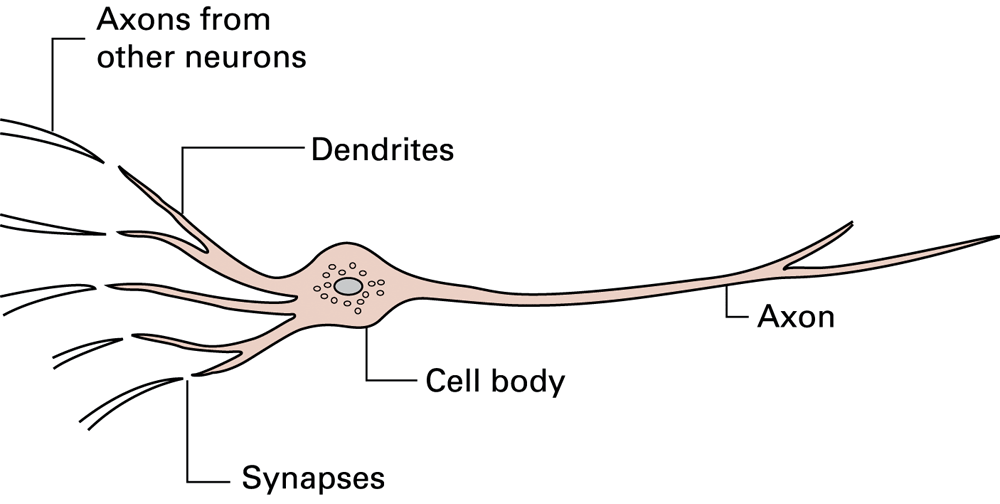
\includegraphics[width=0.7\linewidth]{figs/neuronabio.png}\\
	A neuron has a cell body ...
	\begin{itemize}
	\item ... a branching input structure (dendrite) and 
	\item ... a branching output structure (axon)
	\end{itemize}
	Axons connect to dendrites via synapses
	\smallskip
	\begin{center}
	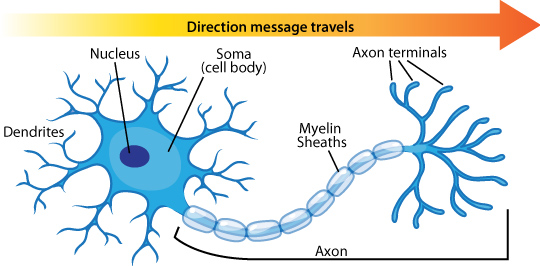
\includegraphics[width=0.6\linewidth]{figs/neuron_anatomy.jpg}
	\end{center}
\end{frame}

\begin{frame}{Advanced AI techniques in videogames}{Artificial Neural Networks (II)} 
\begin{tikzpicture}[scale=0.5,
  init/.style={
   draw,
   circle,
   inner sep=2pt,
   font=\Huge,
   join = by -latex
  },
  squa/.style={
    draw,
    inner sep=2pt,
    font=\Large,
    join = by -latex
  },
	start chain=2,node distance=13mm]
  	\node[on chain=2] 
		  (x2) {$x_2$};
	\node[on chain=2,join=by o-latex] 
		  {$w_2$};
  	\node[on chain=2,init] (sigma) 
		  {$\displaystyle\Sigma$};
	\node[on chain=2,squa,label=above:{\parbox{2cm}{\centering Activate \\ function}}]   
		  {$g$};
  	\node[on chain=2,label=above:Output,join=by -latex] 
		  {$y$};
	\begin{scope}[start chain=1]
		\node[on chain=1] at (0,1.5cm) 
		  (x1) {$x_1$};
		\node[on chain=1,join=by o-latex] 
		  (w1) {$w_1$};
	\end{scope}
	\begin{scope}[start chain=3]
		\node[on chain=3] at (0,-1.5cm) 
		  (x3) {$x_3$};
	  	\node[on chain=3,label=below:Weights,join=by o-latex] 
	   	  (w3) {$w_3$};
	\end{scope}
	\node[label=above:\parbox{2cm}{\centering Bias \\ $W_{0}$}] at (sigma|-w1) (b) {};

	\draw[-latex] (w1) -- (sigma);
	\draw[-latex] (w3) -- (sigma);
	\draw[o-latex] (b) -- (sigma);

	\draw[decorate,decoration={brace,mirror}] (x1.north west) -- node[left=10pt] {Inputs} (x3.south west);
	\end{tikzpicture}

	\bigskip
    \begin{columns}
 	   \column{.70\textwidth}
		\begin{description}
		\item[$a_j$] Normalized input ($0 \le a_j \le 1$)
		\item[$W_{j}$] Weight of input $j$ ($0 \le W_{j} \le 1$)
		\item[$W_{0}$] Bias
		\item[$g$] Activation function
		\end{description}

 	   \column{.30\textwidth}
	   \centering Neuron model
	   \begin{equation*}
	   a_i=g\left( \sum_{j=0}^n W_{j,i} a_j \right)
	   \end{equation*}
    \end{columns}
\end{frame}

\begin{frame}{Advanced AI techniques in videogames}{Artificial Neural Networks (III)} 
\begin{tikzpicture}[shorten >=1pt,->,draw=black!50, node distance=\layersep]
    \tikzstyle{every pin edge}=[<-,shorten <=1pt]
	\tikzstyle{neuron}=[circle,fill=black!25,minimum size=17pt,inner sep=0pt]
	\tikzstyle{input neuron}=[neuron, fill=green!50];
	\tikzstyle{output neuron}=[neuron, fill=red!50];
	\tikzstyle{hidden neuron}=[neuron, fill=blue!50];
	\tikzstyle{annot} = [text width=4em, text centered]

	% Draw the input layer nodes
	\foreach \name / \y in {1,...,4} 
	% This is the same as writing \foreach \name / \y in {1/1,2/2,3/3,4/4} 
	\node[input neuron, pin=left:Input \#\y] (I-\name) at (0,-\y) {};
	% Draw the hidden layer nodes 
	\foreach \name / \y in {1,...,5} 
	\path[yshift=0.5cm] 
	node[hidden neuron] (H-\name) at (\layersep,-\y cm) {}; 
	% Draw the output layer node 
	\node[output neuron,pin={[pin edge={->}]right:Output}, right of=H-3] (O) {}; 
	% Connect every node in the input layer with every node in the 
	% hidden layer. 
	\foreach \source in {1,...,4} 
	\foreach \dest in {1,...,5} 
	\path (I-\source) edge (H-\dest); 
	% Connect every node in the hidden layer with the output layer 
	\foreach \source in {1,...,5} 
	\path (H-\source) edge (O); 
	% Annotate the layers 
	\node[annot,above of=H-1, node distance=1cm] (hl) {Hidden layer}; 
	\node[annot,left of=hl] {Input layer}; 
	\node[annot,right of=hl] {Output layer};
	\end{tikzpicture}
	\\ \href{https://www.youtube.com/watch?v=qv6UVOQ0F44&}{(Video Mario ANN)}
\end{frame}

\subsection{Genetic Algorithms}
\begin{frame}{Advanced AI techniques in videogames}{Genetic Algorithms (I)} 
	Large number of Evolutionary Algorithms
	\begin{itemize}
		\item There is no ``canonical'' algorithm
		\item They all imitate biological evolution
		\item Stochastic search (interesting for videogames)
	\end{itemize}
	They use a population
	\begin{itemize}
		\item Each individual represents a (potential) solution
	\end{itemize}
	Population is modified
	\begin{itemize}
		\item Mutation and crossover
	\end{itemize}
	Selection that imitates natural selection
	\begin{itemize}
		\item Based on a \textbf{fitness} function
	\end{itemize}
	Iterative process
\end{frame}

\begin{frame}{Advanced AI techniques in videogames}{Genetic Algorithms (II)} 
	\begin{center}
		Possible basic algorithm
		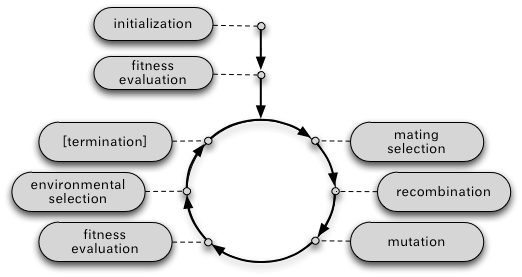
\includegraphics[width=0.75\linewidth]{figs/evolution.png}
	\end{center}
	\href{http://rednuht.org/genetic_cars_2/}{(Demo)}
\end{frame}



\end{document}
